\documentclass[12pt]{extarticle}
\usepackage[utf8]{inputenc}
\usepackage{cite}
\usepackage{graphicx}
\usepackage{float}

\title{Vizualizáció }
\author{Prósz Aurél}
\date{January 2019}

\begin{document}

\maketitle

\section{Tudományos adatok két és háromdimenziós megjelenítésének technikái}
Többdimenziós tudományos adatok megjelenítésére számos módszer áll rendelkezésre, a továbbiakban ezeket szedtem össze kis magyarázat és példa keretében. \newline
Tekintsünk egy példa adatkészletet, például az úgynevezett \textit{Wine Quality Data Set}-et, amely letölthető innen:  https://archive.ics.uci.edu/ml/index.php. Az adatkészlet a portugál \textit{Vinho Verde} bor tulajdonságait írja le, és ezen mutatom be a vizualizációs technikákat. 



    


\subsection{1D és 2D vizualizáció}
Egy dimenzióban, amennyiben egy változó eloszlására vagyunk kiváncsiak, ábrázolhatjuk az adatot \textbf{hisztogramként}. Ha egyszerre több változót kívánunk ábrázolni, úgy lehetőség van őket egyenként elrendezni egy rácson. 

\begin{figure}[H]
    \centering
    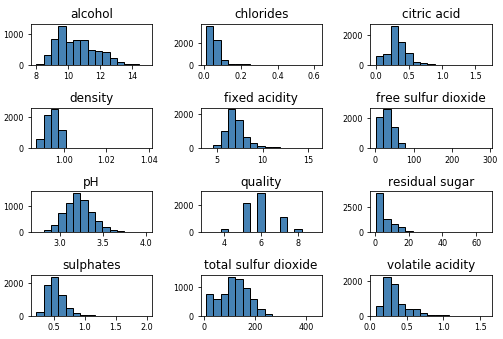
\includegraphics[width=8cm, height=6cm]{hist.png}
    \caption{\textbf{1D adatok ábrázolása hisztogramként.}}
    \label{fig:GeneralDiagram}
 \end{figure}
 
 Egyszerű módszer az adatokon belüli mintázatok és korrelációk felfedezésére az úgynevezett korrelációs módszer kiszámítása, majd annak vizualizációja \textbf{heatmap} formájában. A heatmap esetében az adott párokhoz tartozó értékek jelzik a korreláció, vagy általános esetben bármilyen skalár értékű függvény nagyságát.
 
 \begin{figure}[H]
    \centering
    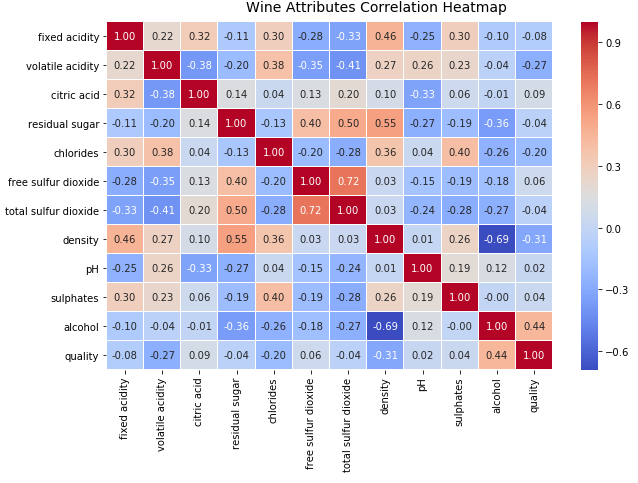
\includegraphics[width=8cm, height=6cm]{kormap.png}
    \caption{\textbf{Korrelációs mátrix megjelenítése heatmap formájában.}}
    \label{fig:GeneralDiagram}
 \end{figure}
 
 Két változó közötti összefüggés megjelenítésére alkalmas a \textbf{scatterplot}, míg a hisztogramokhoz hasonlóan több változó esetén ezt is megjeleníthetjük egy rácson.
 
 \begin{figure}[H]
    \centering
    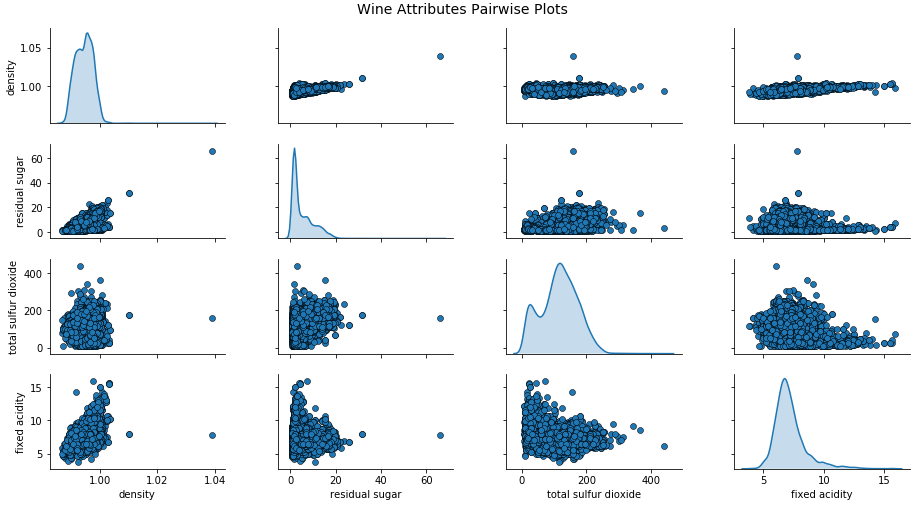
\includegraphics[width=8cm, height=6cm]{pariwise.png}
    \caption{\textbf{Scatterplotok megjelenítése rácson.}}
    \label{fig:GeneralDiagram}
 \end{figure}
 
Több dimenziós, kategorikus adat megjelenítésére szolgál az úgynevezett \textbf{multiple bar plot}, ahol egy klasszikus bar ploton tudunk megjeleníteni több változót is.

\begin{figure}[H]
    \centering
    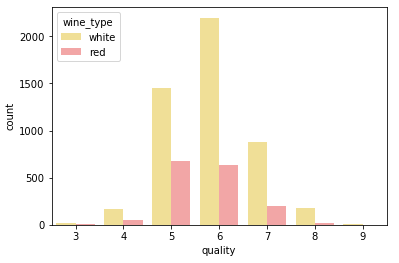
\includegraphics[width=8cm, height=6cm]{multiplebar.png}
    \caption{\textbf{Multiple bar plot két változóval.}}
    \label{fig:GeneralDiagram}
 \end{figure}

A \textbf{box plot} több információt tartalmazó változata a \textbf{violin plot}, amely többváltozós adatot vizualizál olyan módon, hogy az eloszlás alakja is leolvasható az outlier adatpontokkal együtt.


\begin{figure}[H]
    \centering
    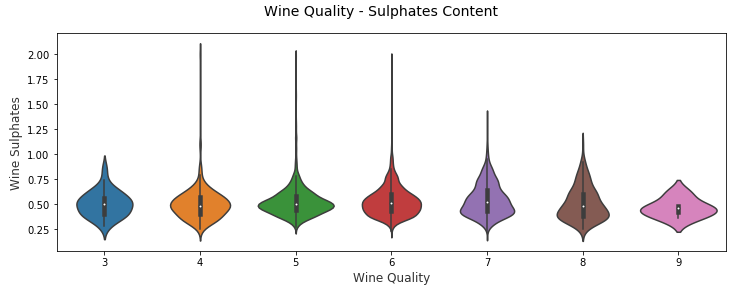
\includegraphics[width=8cm, height=6cm]{violin.png}
    \caption{\textbf{Violin plot több változóval és kategorikus szinezéssel.}}
    \label{fig:GeneralDiagram}
 \end{figure}


\subsection{3D adatvizualizáció}
Amennyiben egyszerre 3 változót szeretnénk megjeleníteni, lehetőségünk van alkalmazni a már korábban látott \textbf{scatterplot}-ot egy rácson elhelyezve, de színkódolás segítségével újabb változó értékét megjeleníthetjük.

\begin{figure}[H]
    \centering
    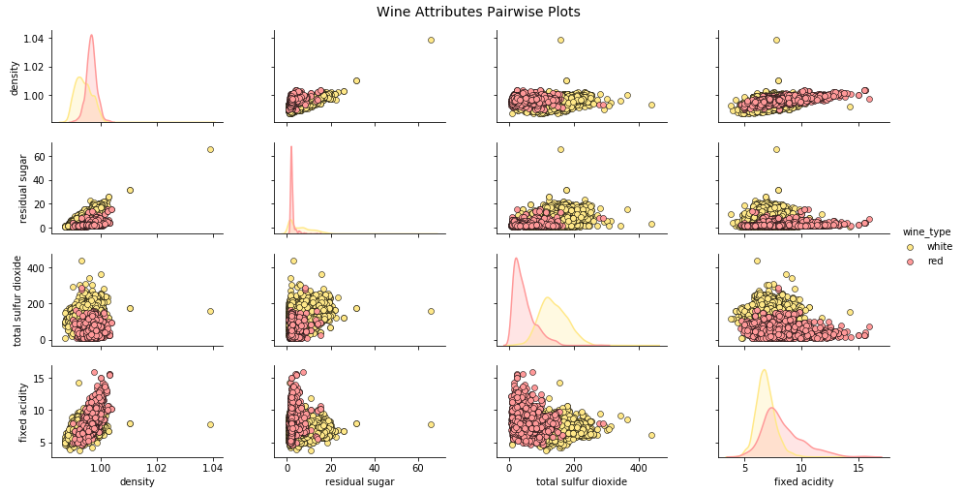
\includegraphics[width=8cm, height=6cm]{3dscatter.png}
    \caption{\textbf{2D scatterplot rácson színkóddal.}}
    \label{fig:GeneralDiagram}
 \end{figure}
 
 Ha mind a három változónk folytonos, akkor érdemes az úgynevezett \textbf{3D scatterplot}-on ábrázolni, amelyben az adatpontok mélységében tároljuk a plusz információt a kétdimenziós megjelenítéshez képest.
 
 \begin{figure}[H]
    \centering
    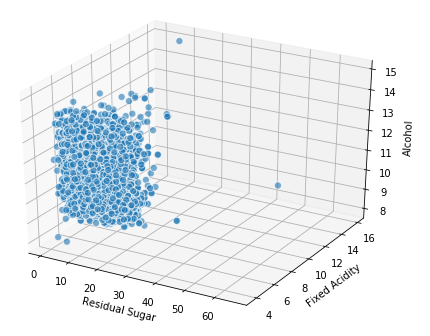
\includegraphics[width=8cm, height=6cm]{3dcont.png}
    \caption{\textbf{3D scatterplot.}}
    \label{fig:GeneralDiagram}
 \end{figure}

 Magasabb dimenzióban az eddigiek analógiájára bővíthetjük a megjelenítést újabb színkódolás, forma, méret, vagy egyéb paraméterek bevezetésével. \newline
 Bővebb információkért, illetve egzotikusabb vizualizációs technikákért érdemes megtekinteni a következő linket: https://towardsdatascience.com/the-art-of-effective-visualization-of-multi-dimensional-data-6c7202990c57
 
 \section{Skalár-, vektor- és tenzorértékű adatok ábrázolása}
 https://booksite.elsevier.com/samplechapters/9780123875822/9780123875822.PDF
 \subsection{Skalár értékű adatok ábrázolása}
 
 Skalár értékű adatokat az előző részekben tárgyaltakon kívül ábrázolhatunk még felületeken, vagy térfogatokban olyan módon, hogy színekkel jelöljük a konkrét értékeket, ezt nevezzük \textbf{color mapping}-nak. \newline
 Másik módszer az úgynevezett \textbf{contouring}, amely egyfajta kibővítése a color mapping-nak olyan módon, hogy a szinte azonos színű (és értékű) régiókat kontúrvonalakkal (vagy kontúrfelületekkel) elkeríti, és ezeket a területeket (vagy térfogatokat) ugyanolyan színnel színezi. Tipikus példa erre a megjelenítsére az időjárást ábrázoló térképek, ahol a konstans hőmérsékletet jellemző kontúrvonalak választják el az egyes régiókat.
 
 \begin{figure}[H]
    \centering
    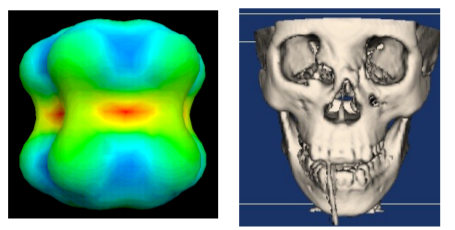
\includegraphics[width=8cm, height=6cm]{iso.PNG}
    \caption{\textbf{Példa a kontúrvonalakra és a kontúrfelületekre.}}
    \label{fig:GeneralDiagram}
 \end{figure}
 
 \subsection{Vektor értékű adatok ábrázolása}
 Vektor értékű adatok adatok ábrázolását a legegyszerűbb módon úgy valósíthatjuk meg, hogy minden egyes adatponthoz társítunk egy vonalat, amelynek meghatározott iránya és nagysága van. A technika neve \textbf{hedgehog}, a keletkező vizualizáció kinézete miatt. A megjelenítést tovább lehet finomítani a vonalak színezésével és méretük változtatásával. Ezen kívül az egyszerű vonalak helyett alkalmazhatunk 2D és 3D irányított objektumokat is, amelyek többdimenziós adatok megjelenítésénél lehet hasznos, mert könnyebb a jelölt irányt megállapítani az alkalmazásukkal.
 
 \begin{figure}[H]
    \centering
    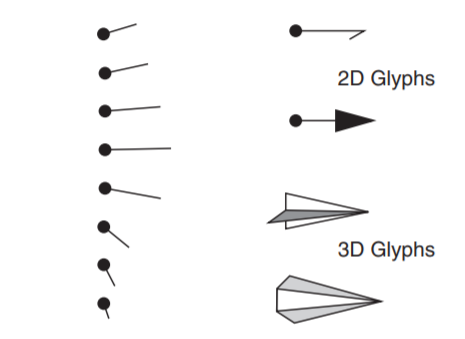
\includegraphics[width=8cm, height=6cm]{glyph.PNG}
    \caption{\textbf{Példa az egyszerű vonalas vektorábrázolásra, illetve a bonyolultabb 2D és 3D objektumok használatára.}}
    \label{fig:GeneralDiagram}
 \end{figure}
 
 A vektor értékű adatok ábrázolásánál figyelni kell, hogy 3 dimneziós ábrázolásoknál sokszor nehéz pontosan megállapítani a vektorok irányítottságát, hiszen a 3D térből vetítjük le a megjelenítést a 2D térbe. Ezen kívül fontos, hogy ne jelenítsünk meg egyszerre túl sok adatpontot, mert a vektorok összemosódhatnak és értelmezhetetlenné válik az ábra. 
 
  \subsection{Tenzor értékű adatok ábrázolása}
 TODO
 \section{Színek}
 Tudományos publikációkban rendkívül fontos szerepe van a megfelelő színválasztásnak. Ehhez előre definiált színpaletták állnak rendelkezésre, a következőkben ezeket tekintem át. Általános alapelv a színválasztásnál, hogy a megjelenített adatokat egyértelművé tegye, ne torzítsa el, és az esetleges színtévesztő olvasók számára is problémamentes legyen a megjelenítés.
 
 \subsection{Szekvenciális adatok színezése}
 
 Amennyiben olyan adatot kívánunk megjeleníteni, amely értékei folytonosak és sorba rendezhetőek nagyság szerint, úgy érdemes az úgynevezett szekvenciális paletták közül válogatni. Ennek előnye, hogy a legtöbb ember a sötétebb színeket, például a feketét a "több", vagy "sűrűbb" adathoz társítja, míg a világosabb színek az ellenkező hatást érik el. 
 
 \begin{figure}[H]
    \centering
    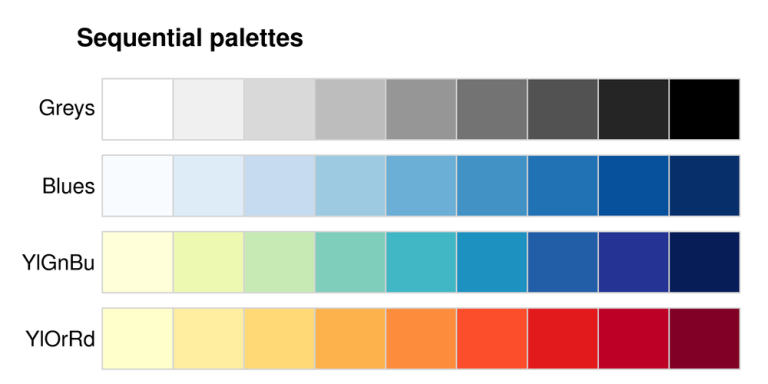
\includegraphics[width=8cm, height=6cm]{sequential.png}
    \caption{\textbf{Szekvenciális paletták}}
    \label{fig:GeneralDiagram}
 \end{figure}
 
  \begin{figure}[H]
    \centering
    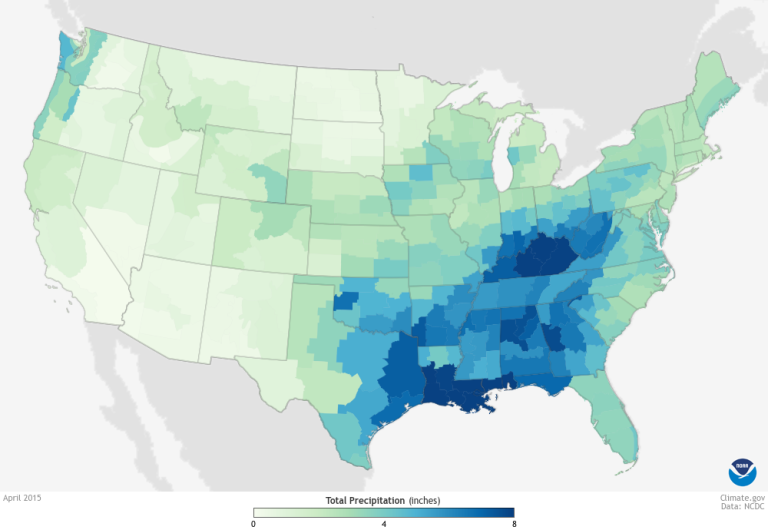
\includegraphics[width=8cm, height=6cm]{map.png}
    \caption{\textbf{Egy példa a szekvenciális adatok színezésére.}}
    \label{fig:GeneralDiagram}
 \end{figure}
 \subsection{Divergens adatok színezése}
 Ha az adataink divergens struktúrájúak, tehát tartozik hozzá egy nullpont, amihez képest lehet az adatok értéke nagyobb, vagy kisebb, akkor célszerű a divergens színpalettákból válogatni. Ezek olyan paletták, amelyek két vége tendál a sötétebb színek felé, így mutatva, hogy azok a részei a "jobban" negatívak, vagy pozitívak.
 
  \begin{figure}[H]
    \centering
    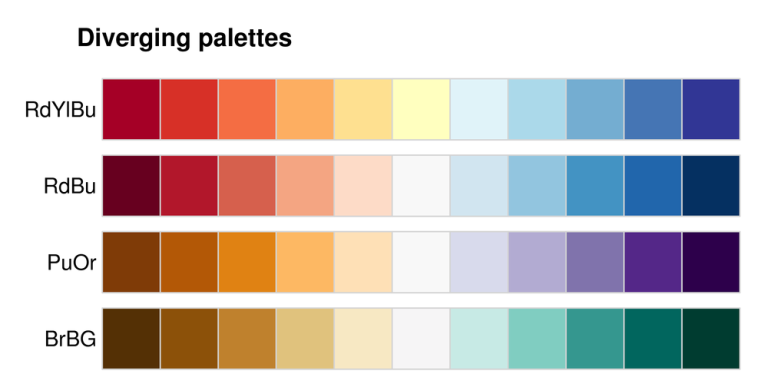
\includegraphics[width=8cm, height=6cm]{diverging.png}
    \caption{\textbf{Divergens paletták}}
    \label{fig:GeneralDiagram}
 \end{figure}
 
 \subsection{Kategorikus adatok színezése}
 Kategorikus adatok esetében, amelyek nem állíthatóak sorba, törekednünk kell arra, hogy egymástól jól megkülönböztethető színeket használjunk, illetve, hogy egy ábrázoláson csak megfelelő mennyiségű kategóriát szerepeltessünk, hogy ne legyenek összekeverhetőek az adatpontok.
 
 
 
 \begin{figure}[H]
    \centering
    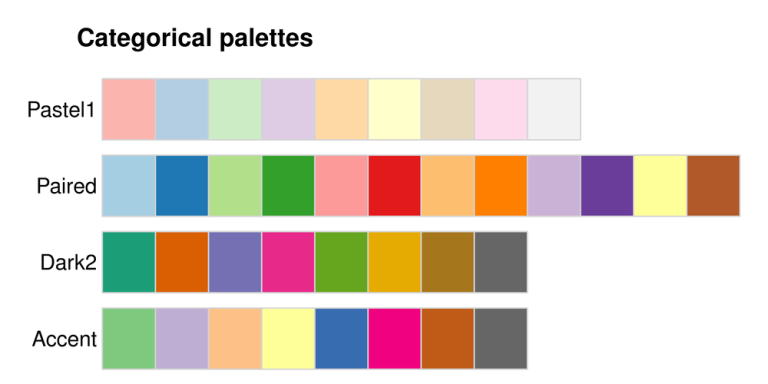
\includegraphics[width=8cm, height=6cm]{categorical.png}
    \caption{\textbf{Kategorikus paletták}}
    \label{fig:GeneralDiagram}
 \end{figure}
 
 \subsection{Egyéb szempontok}
 
 Fontos szempont, hogy az adatok megjelenítésénél gondoljunk  színtévesztő olvasókra. Ehhez általános szabály, hogy pirosat és zöldet soha ne használjunk együtt, mert a színtévesztés leggyakoribb fajtája (8\% férfiaknál, 0.5\% nőknél) pont ezt a két színt teszi nehezen megkülönböztethetővé. Ezen szabály betartása mellett rendelkezésre állnak kifejezetten színtévesztőknek kifejlesztett színpaletták is, ezek használata is indokolt lehet. 
 
 \begin{figure}[H]
    \centering
    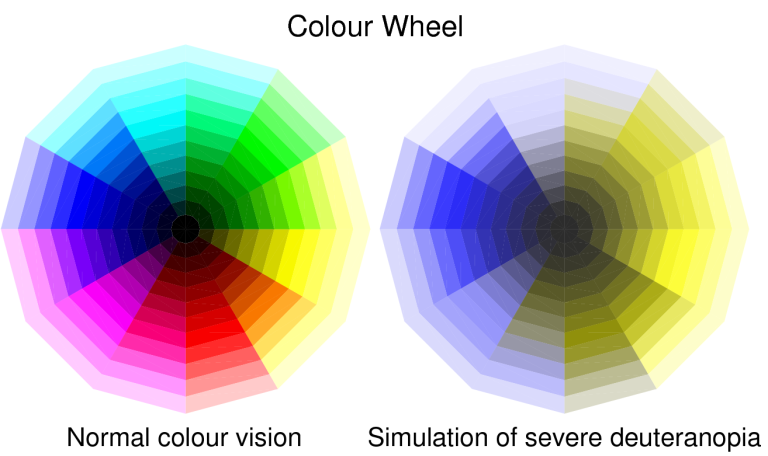
\includegraphics[width=8cm, height=6cm]{cwheel-polar.png}
    \caption{\textbf{Színtévesztés szimulálása.}}
    \label{fig:GeneralDiagram}
 \end{figure}
 
 \begin{figure}[H]
    \centering
    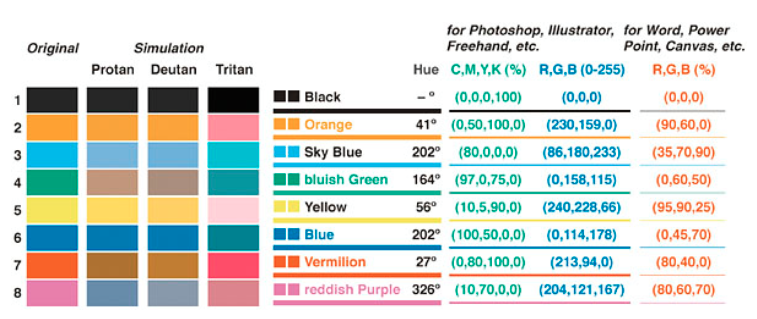
\includegraphics[width=8cm, height=6cm]{colorb.png}
    \caption{\textbf{Színtévesztő-barát színpaletták}}
    \label{fig:GeneralDiagram}
 \end{figure}
 
 \newline

 \section{Térbeli adatok megjelenítése, volometrikus és szintfelületes ábrázolás.}
 TODO
 
 \section{Háromdimenziós renderelési technikák, ray casting, ray tracing.}
 TODO
 
 

 
  
\section{A sztereoszkópius megjelenítés technológiái}

Sztereoszkópiának hívunk bármilyen olyan technológiát, amely lehetőséget ad egy 2D kép olyan módon való megjelenítésére, amely valódi 3D képnek tűnő hatást kelt. Fotók, vagy videók esetében ezt úgy érik el, hogy különböző képet mutatnak a különböző szemeknek. \newline
A térlátás abból adódik, hogy az emberi szemek közelítőleg 5 cm-re helyezkednek el egymáshoz képest, így egy adott jelenséget a két szem kicsit más szögből látja. Lehetőség van ennek analógiájára olyan kamerát készíteni, amely két lencsével rendelkezik, reprodukálva az emberi látás sajátosságait. Alapvetően kétfajta technikát különböztetünk meg: a sztereoszkópikus és az autosztereoszkópikus megjelenítéseket. Az elsőnél a megfigyelőnek szüksége van valamilyen eszköz, például speciális szemüveg viselésére a 3D hatás megtapasztalására, míg a másodiknál nincs. \newline
\subsection{Anaglif megjelenítés}
A sztereoszkópikus technológia felbontható több csoportra. Az első ilyen módszer az úgynevezett anaglif megjelenítés. Ennek során egy képet két különböző szögből vesznek fel, majd két különböző színnel látnak el, amelyet hasonló színezésű szemüveggel (egy szín az egyik, másik szín a másik szemnek) vizsgálva előhozható a 3D megjelenítés. Általában a két használt szín a piros és a kék. Előnyei a technikának, hogy nagyon egyszerűen lehet előállítani a kompozit képet, és olcsó a hozzá tartozó szemüveg. Ezen kívül fizikailag is kinyomtatható a kép, a hatás úgy is megmarad. Hátrányai, hogy nehéz valódi színeket megjeleníteni rajta, a keletkező kép gyakran homályos.

\begin{figure}[H]
    \centering
    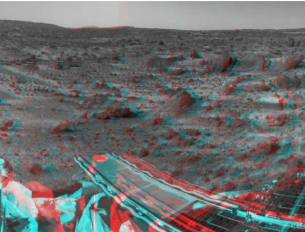
\includegraphics[width=8cm, height=6cm]{stereo.PNG}
    \caption{\textbf{Anaglif kép.}}
    \label{fig:GeneralDiagram}
 \end{figure}



\subsection{Polarizációs szemüvegek}

Ez a technika hasonló az anaglif megjelenítéshez, de itt színkódolás helyett különböző polarizációs szűrőkön vezetik át a két szemhez tartozó képet. Előnye az előzőhöz képest a jobb színhűség, de hátránya, hogy a megjelenő kép homályos és fényszegény a szűrők fényelnyelése miatt.

\subsection{Shutter szemüvegek}

Ennek a technika során a speciális szemüveg periodikusan kitakarja egyszer az egyik, másszor a másik szem képét, így a kijelző videokártyájával megfelelően szinkronizálva, majd azon megfelelő időben megjelenítve a képeket elérhető a 3D hatás. Előnye, hogy sokkal meggyőzőbb képet ad az előző két technikával szemben, de hátránya, hogy a speciális szemüvegek gyakran nagyon drágák, és értelemszerűen a keletkező képet kinyomtatni se lehet. \newline
\subsection{Autosztereoszkópikus technikák}
Az autosztereoszkópikus technikák is felbonthatóak több csoportra. 
 
https://www.cg.tuwien.ac.at/courses/Seminar/WS2006/stereo_techniques.pdf

\section{Számítógépes geometria}
TODO
\bibliographystyle{plain}
\bibliography{M335}

\end{document}
